%%%%%%%%%%%%%%%%%%%%%% EXPERIMENTS %%%%%%%%%%%%%%%%%%%%%%
\subsection{Experimental Setup}\label{sec:experiments}

\subsubsection{Training and Evaluation Corpora} 
%
A corpus is collected in a PyBullet tabletop environment using a simulated Franka Emika Panda robot arm~\citep{haddadin2022franka}. The training data set for neural predictor and discriminator consists of a corpus of $3000+$ initial and final world states along with a single-step natural language instruction. 
%
Scenes correspond to a tabletop workspace with $3-5$ blocks of varying colors and shapes and placed at randomized world locations. 
%
To evaluate error-recovery, a data set of $2000+$ robot executions with errors is generated. The following types of errors are introduced during the plan execution (i) random application of force on an object (ii) external agent intervention that interchanges the location of any two objects. The instructions consist of $1-10$ step actions, the scenes have $5-10$ objects 
with a maximum of $5$ errors introduced at a single step. The dataset is divided into 3 splits as detailed in table \ref{tab:eval-error}.

\begin{table}[]
    \centering
    \begin{tabular}{|c|c|c|c|c|}
         \hline
         \textbf{Dataset} & \textbf{Num objects} & \textbf{Num steps} & \textbf{Num errors} & \textbf{Size} \\
         \hline
         Dataset 1 & Fixed (5) & Fixed (5) & \textbf{Varying} (1-5 on a random step) & 773  \\
         Dataset 2 & Fixed (5) & \textbf{Varying} (1-8) & Fixed (1 error per step) & 1316 \\
         Dataset 3 & \textbf{Varying} (6-10) & Fixed (10) & Fixed (5 on a random step) & 215 \\ 
         \hline
    \end{tabular}
    \caption{Evaluation Datasets}
    \label{tab:eval-error}
\end{table}

% \begin{enumerate}
%     \item \textbf{Dataset 1.} 5 objects in scene, 5 step plan, and varying number of errors (1 – 5) on a random step
%     \item \textbf{Dataset 2.} 5 objects in scene, single error per step, and varying number of steps in the plan (1 – 8) 
%     \item \textbf{Dataset 3.} 10 step plan, 5 errors on a random step, and varying number of objects in the scene (6 – 10)
% \end{enumerate}


\subsubsection{Baselines and Ablations}\label{subsec:baseline}
The proposed approach is compared with two baseline approaches: \begin{enumerate}
    \item \emph{RePlan:} a neuro-symbolic planner inspired from \cite{mao2022pdsketch} that uses A$^*$-search as its planning framework. This planner uses a transition function and the goal-check function. Even though it can detect whether or not it has reached the goal-state, it lacks the reasoning to detect whether an error has occurred at some intermediate state or not. For a fair comparison the baseline is augmented with the discrepancy predictor (in the form of our $=_\mathcal{Z}$) and a domain-specific heuristic ($\mathcal{D}$).
    \item \emph{NoFree:} our planner except the \textit{free}-space transformer network. Even though this planner is \textit{discrepancy}-aware, the action space is large and cannot be effectively pruned in general settings as it lacks the ability to reason over the metric-space (for block un-stacking etc.) which otherwise was not needed due to the \textit{free}-space transformer inspired from~\citep{liu2022structdiffusion}.
\end{enumerate}

We also evaluated an RL-based reactive planner ~\citep{li2020towards}. The learned goal-conditioned policies performed poorly (after $12$ hours of training) in terms of goal-reaching rate, attributed largely to the domain complexity. 

For a fair comparison, the action pre-conditions and object association between different states is known. 

%%%% Metrics for evaluating error recovery
\subsubsection{Evaluation Metrics} 
We adopt the following metrics:
\begin{enumerate}
    \item \textit{Detection Accuracy}: Detecting if the current state after an action execution is erroneous 
    \item \textit{Recovery Accuracy}: Given correct detection, generating a correct recovery plan which on execution leads to the intended intermediate state
    \item \textit{Length efficiency $(L_{plan}/L_{opt})$}: Ratio of the returned recovery plan length $L_{plan}$ to the length of the most optimal recovery plan possible $L_{opt}$.
    \item \textit{Time efficiency $(T_{plan}/L_{opt})$}: To evaluate if the recovery planning is fast. It is the ratio of the planning time $T_{plan}$ to the length of the most optimal recovery plan possible $L_{opt}$, and measures the time taken per unit optimal plan length.
    \item \textit{Fraction of plan completed}: Evaluating the fraction up to which the original plan could be completed by successfully recovering from errors.
\end{enumerate}

%%%%%%%%%%%%%%%%%%%%%% RESULTS %%%%%%%%%%%%%%%%%%%%%% 
\subsection{Results}\label{sec:results}
Our experiments evaluate (i) effectiveness of the model in error recovery in relation to alternative approaches, (ii) an analysis of model components, (iii) effectiveness in relation to increase in in plan length and compounding of errors, increase in number of objects in the scene, and recovering from multiple errors, 
%(iv) anytime version of the model, 
and (iv) qualitative results on a simulated Franka Emika Robot operating in a table top environment. 

\subsubsection{Plan Recovery with Single-step Errors} 
We consider the setting where recovery is needed once during the whole execution as a result of multiple errors introduced together. Table \ref{tab:dset1} reports the performance of various models on Dataset 1. Note that recovery accuracy is reported for cases where error detection is correct, and the efficiency metrics are reported when the recovery plan is correct as well. Our model generates a recovery plan significantly quicker compared to the other two models, due to its discrepancy-awareness and effective action pruning from the free-space network. The low recovery time contributes to a high recovery accuracy, due to the presence of an overall time budget ($\sim$60s).

\begin{table*}
    \centering
    \caption{Performance comparison with multiple errors introduced at a single step.}
    \begin{tabular}{|l|c|c|c|c|}
    \hline
         Model & Recovery \% &  $L_{plan}/L_{opt}$ & $T_{plan}/L_{opt}$  \\ 
         \hline
         \hline
         Ours & \textbf{99.61} & 1.13 & \textbf{0.06s} \\ 
         \hline 
         RePlan & 96.89 & 1.12 & 0.22s \\
        \hline 
         NoFree & 87.83 & 1.05 & 0.42s \\ 
         \hline
    \end{tabular}
    \label{tab:dset1}
\end{table*}

%
\subsubsection{Plan Recovery with Compounding Errors}
%
We now consider a setting where a single error is introduced at each step of a multi-step plan. Table \ref{tab:dset2} reports the performance of various models on Dataset 2. Our model is able to recover a significantly higher part of the original plan due to its high recovery accuracy, which in turn is due to its fast planning capabilities.
%

\begin{table*}
    \centering
    \caption{Performance comparison when errors compound over time. }
    \begin{tabular}{|l|c|c|c|}
    \hline
         Model & Recovery \% & Completion \% \\ 
         \hline
         \hline
         Ours & \textbf{99.24} & \textbf{99.68} \\ 
         \hline 
         RePlan & 93.54 & 96.86 \\
        \hline 
         NoFree & 66.49 & 78.05 \\ 
         \hline
    \end{tabular}
    \label{tab:dset2}
\end{table*}

%
\subsubsection{Evaluation of Model Components}
%
Table \ref{tab:model-comp} summarises the evaluation of various model components. Error detection has a fairly high accuracy demonstrating a high accuracy of scene-graph predictor and discriminator, however high recall and relatively low precision indicates the model is susceptible to false positives, leading to unnecessary re-tries and recovery plans when there are no errors. The accuracy for precondition detection is also high, but relatively low recall indicates the presence of false negatives, disallowing feasible actions leading to longer recovery plans or even failures.

\begin{table*}
    \centering
    \begin{tabular}{|l|l|c|}
    \hline
    Component & Metric & Performance\\
    \hline
    \hline
    Error detection & Accuracy & 94.54\%\\
    & Recall & 0.99\\
    & Precision & 0.79\\
    \hline
    Precondition detection & Accuracy & 94.19\% \\
    & Recall & 0.93\\
    & Precision & 0.99\\
    \hline
    Object matching & Accuracy & 88.23\% \\
    \hline
    Scene-graph predictor & Accuracy & 96\% \\
    & IoU & 0.84 \\
    \hline
    Scene-graph discriminator & Accuracy & 0.98\\
    \hline
    Free-space transformer & IoU & 0.007\\
    \hline
    \end{tabular}
    \caption{Evaluation of various model components}
    \label{tab:model-comp}
\end{table*}

\subsubsection{Effect of varying number of errors, steps and objects}
%
Figure \ref{fig:graphs-errors} illustrates the effect of more errors being introduced at a single step, measured by longer optimal recovery plans. Our approach generalises well to more errors, maintaining a higher recovery rate and time efficiency compared to the baselines. Even though our approach and RePlan have close successful recovery rate, our approach is approximately 4x faster than RePlan.
%
Figure \ref{fig:graphs-steps} illustrates the effect of increase in original plan length, with a randomized error introduced at each step. As the original plan becomes longer, the fraction of plan completed decreases which can be attributed to compounding of incorrect error detection and recovery. Our approach generalises better to more number of steps compared to the baselines. 
%
Figure \ref{fig:graphs-obj} shows that our model generalises well to more number of objects in the scene than what is was trained on. Object matching accuracy decreases as the number of objects increase due to the compounding inaccuracy of node and object discriminators.

\begin{figure}
    \begin{subfigure}{0.5\hsize}
       \centering    \includegraphics[width=0.9\textwidth]{assets/vary-errors-1.png}
    \end{subfigure}
    \begin{subfigure}{0.5\hsize}
       \centering    \includegraphics[width=0.9\textwidth]{assets/vary-errors-2.png}
    \end{subfigure}
    \caption{
        Varying number of introduced errors
    }
    \label{fig:graphs-errors}
\end{figure}

\begin{figure}
    \begin{subfigure}{0.5\hsize}
       \centering    \includegraphics[width=0.9\textwidth]{assets/vary-steps-1.png}
    \end{subfigure}
    \begin{subfigure}{0.5\hsize}
       \centering    \includegraphics[width=0.9\textwidth]{assets/vary-steps-2.png}
    \end{subfigure}
    \caption{
        Varying number of steps in the original instruction
    }
    \label{fig:graphs-steps}
\end{figure}

\begin{figure}
    \begin{subfigure}{0.5\hsize}
       \centering    \includegraphics[width=0.9\textwidth]{assets/vary-obj-1.png}
    \end{subfigure}
    \begin{subfigure}{0.5\hsize}
       \centering    \includegraphics[width=0.9\textwidth]{assets/vary-obj-2.png}
    \end{subfigure}
    \caption{
        Varying number of objects in the scene
    }
    \label{fig:graphs-obj}
\end{figure}

\subsubsection{Simulation Results}
Figure \ref{fig:rollout} demonstrates a 5-step instruction with an introduced error provided to a simulated 7-DOF Franka Emika manipulator in a table top setting. An external agent interchanges the location of 2 objects, which is detected using the predicted intermediate scene graph. A 3-step recovery plan is generated, which consists of first moving the yellow dice to a free space, followed by moving the two objects to their correct positions. Figure \ref{fig:error-qualit} shows some more qualitative results of recovery from single-step errors and compounding errors, and a very long recovery plan.
Figure ~\ref{fig:anytime-qual} compares the anytime recovery with the basic ("Ours", recovering to the next intermediate state) approach, for the cooperative agent example introduced earlier (Figure ~\ref{fig:anytime}). The basic approach follows a 2-step recovery plan to the next intermediate state $S_2$, leading to a total of 4 steps to the goal. This involves unnecessary unstacking and restacking of the red cube. In comparison, anytime recovery is able to identify the optimal intermediate state to recover to, which in this case is $S_3$, and performs a 1-step recovery plan leading to just 2 steps to the goal.

\begin{figure}
    % \centering
    \begin{subfigure}{\textwidth}
        \includegraphics[width=\textwidth]{assets/anytime-o.png}
        \caption{Basic approach ("Ours"). Recovery to state $S_2$, leading to total 4 steps to the goal}
    \end{subfigure}

    \vspace{0.5cm}

    \begin{subfigure}{\textwidth}
        \includegraphics[width=0.67\textwidth]{assets/anytime-a.png}
        \caption{Anytime recovery with K=4. Recovery to state $S_3$, leading to just 2 steps to the goal}
    \end{subfigure}
    
    \caption{Basic vs anytime recovery for a cooperative agent. Discrepancies are highlighted via bounding boxes. Recovery steps are denoted in a green background}
    \label{fig:anytime-qual}
\end{figure}

\begin{figure}
    \centering
    \begin{subfigure}{\textwidth}
        \includegraphics[width=\textwidth]{assets/dset1.png}
        \caption{An example from dataset 1. Instruction: "Place the white lego on top of the red lego". An external force and rearrangement is applied, leading to discrepancy in 3 objects, triggering a 4-step recovery plan}
    \end{subfigure}

    \vspace{1cm}

    \begin{subfigure}{\textwidth}
        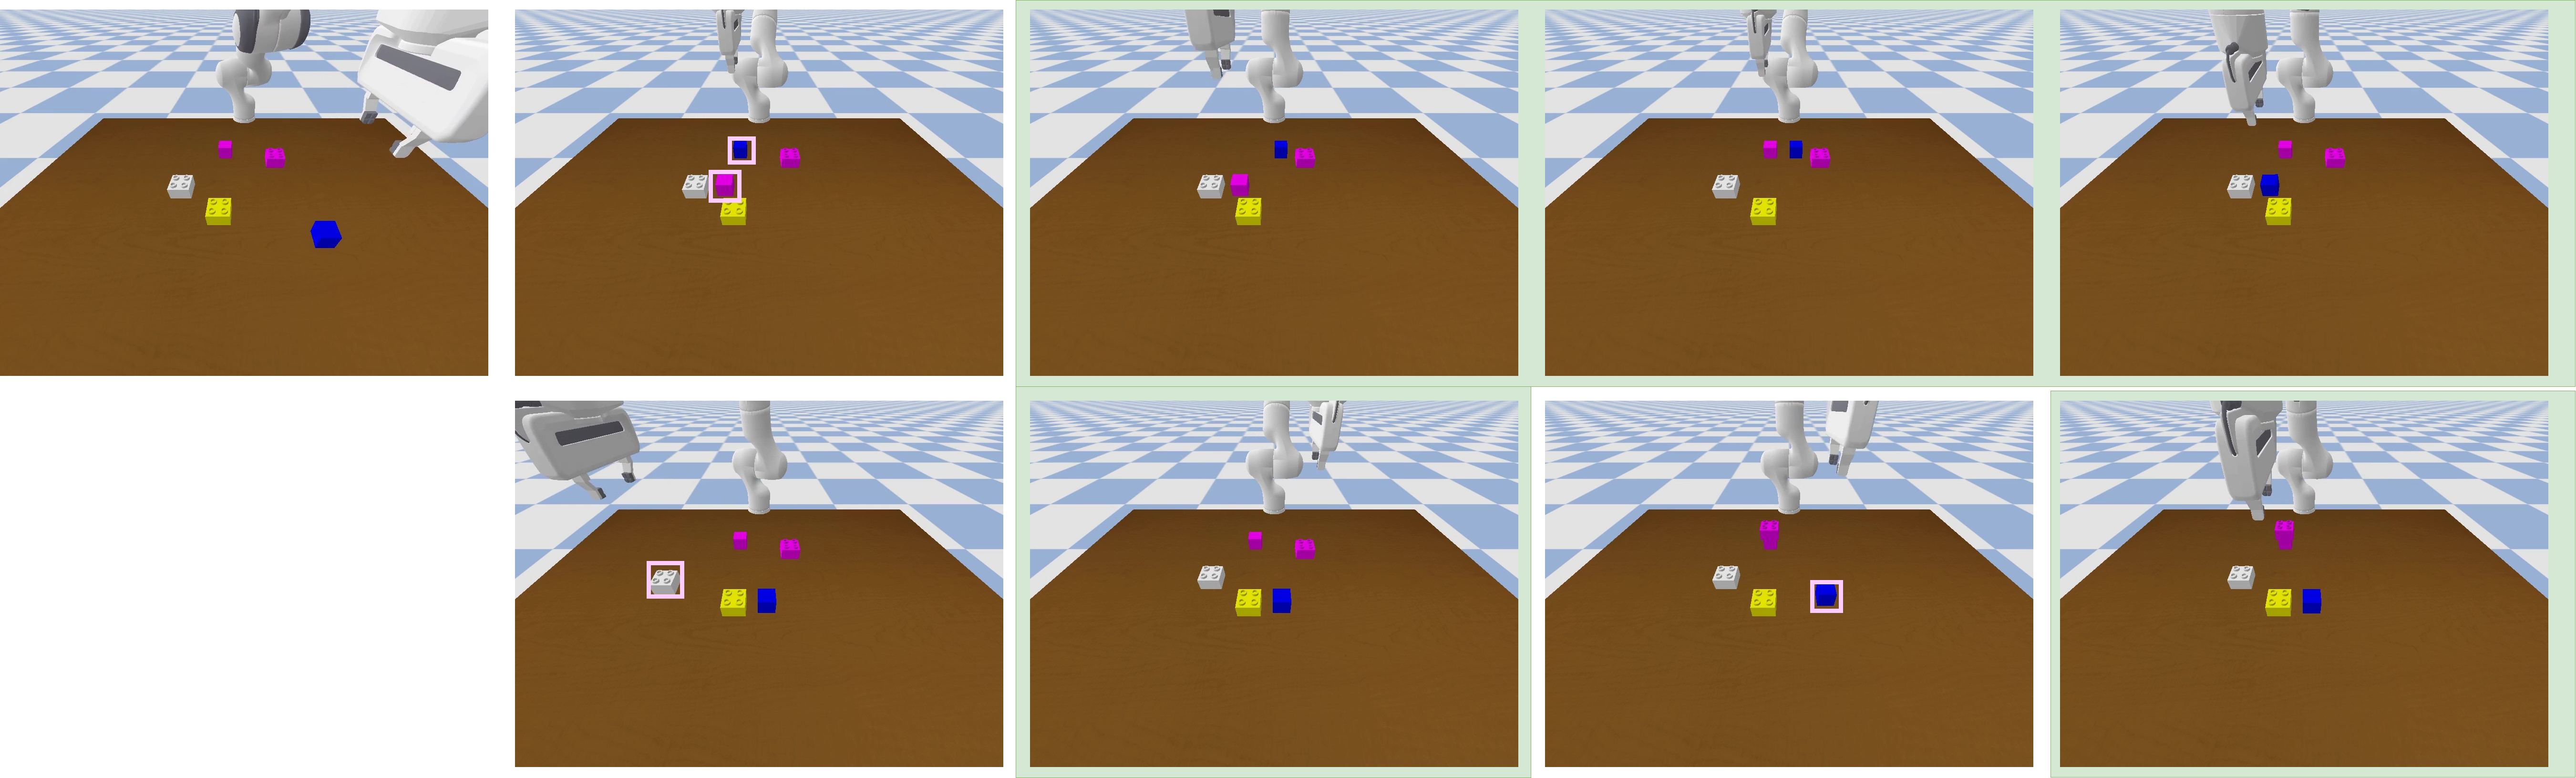
\includegraphics[width=\textwidth]{assets/dset-2.png}
        \caption{An example from dataset 2. 3-step instruction: "Put the blue lego to the right of the white lego and put the blue lego to the right of the yellow lego and put the magenta lego on top of the magenta cube". A  rearrangement on the first step followed by force on subsequent steps leads to recoveries of length 3,1,1 respectively}
    \end{subfigure}

    \vspace{1cm}

    \begin{subfigure}{\textwidth}
        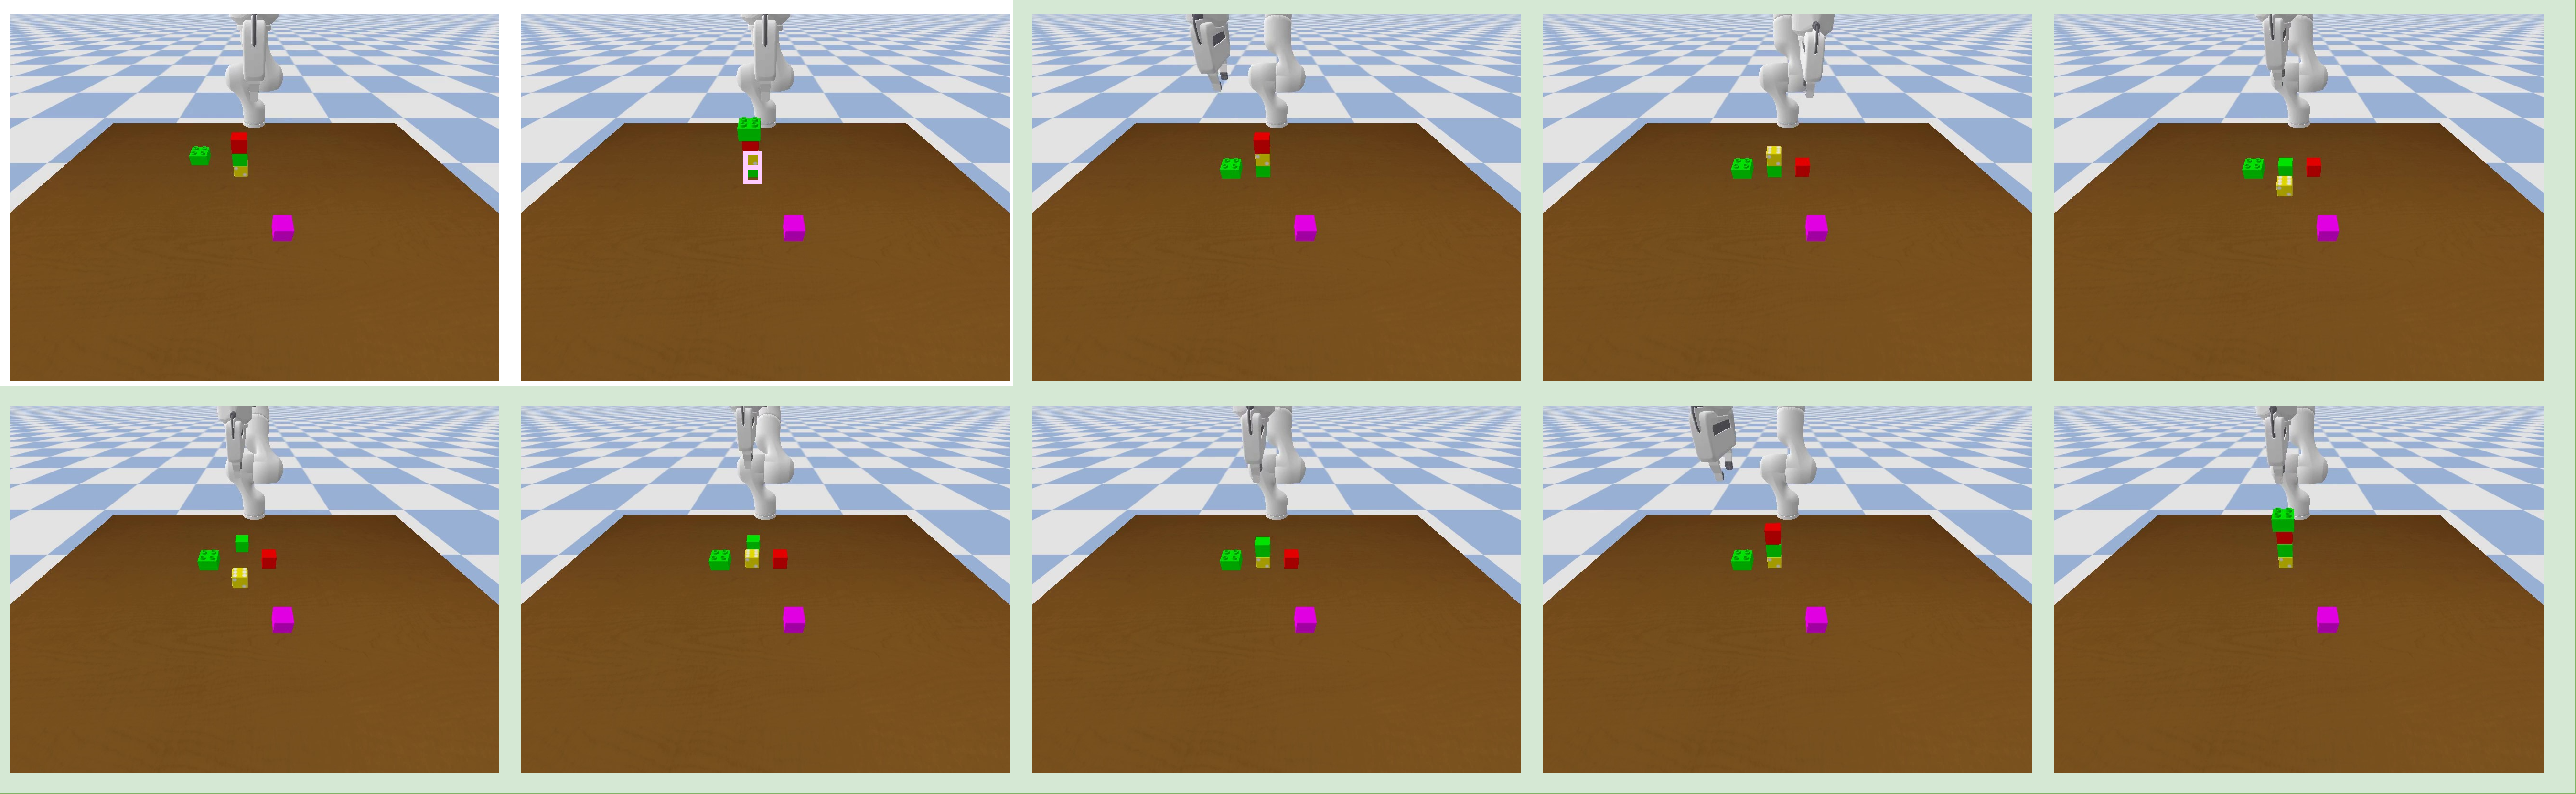
\includegraphics[width=\textwidth]{assets/long.png}
        \caption{A long recovery example. While creating a tower of 4, the bottom two blocks of the tower are interchanged, triggering an 8-step recovery plan.}
    \end{subfigure}

    \vspace{1cm}
    
    
    \caption{Qualitative results for error recovery. Discrepancies are highlighted via bounding boxes. Recovery steps are denoted in a green background}
    \label{fig:error-qualit}
\end{figure}





